\begin{frame}
  \frametitle{Modeling Probabilistic Design}
  \begin{block}{Probabilistic Boolean Network (PBN)}
    A Boolean network with $B_v\sim\textit{Bernoulli}(p_v)$ for each vertex $v$:
    \pause
    \begin{itemize}
      \item Primary inputs: $p_v=\Pr[v=\top]$
            \pause
      \item Other vertices: $p_v$ is the error rate of $v$
    \end{itemize}
  \end{block}
  \pause
  \begin{block}{Example}
    A PBN with $V_I=\{x_1,x_2,x_3\},V_O=\{o\}$:
    \begin{figure}
      \centering
      \begin{circuitikz}[scale=0.7, transform shape]
  % Logic gates
  \node[color=red, and port] (y1) {$y_1$};
  \node[or port, right = of y1, anchor=in 1] (y2) {$y_2$};
  % Wires
  \draw (y1.out) -- (y2.in 1);
  % Labels
  \node[left = 0.1cm of y1.in 1] {$x_1$};
  \node[left = 0.1cm of y1.in 2] {$x_2$};
  \node[left = 0.1cm of y2.in 2] {$x_3$};
  \node[right = 0.1cm of y2.out] {$o$};
\end{circuitikz}
    \end{figure}
    \pause
    \begin{itemize}
      \item $p_{x_1}=p_{x_2}=p_{x_3}=0.5$
            \pause
      \item $p_{y_1}=0.25;p_{y_2}=p_{o}=0$
    \end{itemize}
  \end{block}
\end{frame}

\begin{frame}
  \frametitle{Modeling Probabilistic Design}
  \begin{block}{Standardized Probabilistic Boolean Network (SPBN)}
    A PBN can be standardized by the following \textit{distillation operation}:
    \pause
    \begin{figure}
      \centering
      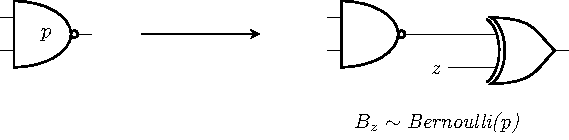
\includegraphics[scale=0.8]{fig/prob-design-eval/prob-distillation.pdf}
    \end{figure}
  \end{block}
  \pause
  \begin{block}{Example}
    A standardized PBN with $V_I=\{x_1,x_2,x_3\},V_O=\{o\}$:
    \begin{figure}
      \centering
      \begin{circuitikz}[scale=0.7, transform shape]
    % Logic gates
    \node[and port] (y1) {$y_1'$};
    \node[xor port,right = of y1, anchor=in 1] (y3) {$y_3$};
    \node[or port,right = of y3, anchor=in 1] (y2) {$y_2$};
    % Wires
    \draw (y1.out) -- (y3.in 1);
    \draw (y3.out) -- (y2.in 1);
    % Labels
    \node[left = 0.1cm of y1.in 1] {$x_1$};
    \node[left = 0.1cm of y1.in 2] {$x_2$};
    \node[left = 0.1cm of y2.in 2] {$x_3$};
    \node[right = 0.1cm of y2.out] {$o$};
    \node[left = 0.1cm of y3.in 2] {$z_1$};
\end{circuitikz}
    \end{figure}
    \pause
    \begin{itemize}
      \item $p_{z_1}=0.25;p_{y_1'}=p_{y_3}=0$
    \end{itemize}
  \end{block}
\end{frame}